\documentclass[12pt]{article}
\usepackage[margin=1in]{geometry}
\usepackage{graphicx,booktabs,url,setspace,caption,amsmath,float}
\usepackage[T1]{fontenc}\usepackage{lmodern}\usepackage[hidelinks]{hyperref}
\captionsetup{font=small,labelfont=bf,justification=justified}
\setstretch{1.15}
\title{Kindergarten MMR Vaccination, Non-Medical Exemptions, and Measles Cases Across U.S. States, 2024 to 2025: An Ecological Analysis}
\author{Haoxi Hu\thanks{Corresponding author: \href{mailto:hu.haoxi@northeastern.edu}{hu.haoxi@northeastern.edu}}\\[2pt]
\small Khoury College of Computer Sciences and Bouv\'e College of Health Sciences,\\
\small Northeastern University}
\date{}
\begin{document}
\maketitle
\vspace{-2em}
\begin{abstract}
Background: Measles spreads easily when vaccination coverage falls below about 95\%, and the United States recorded 2,263 state-reported cases in 2025 after 269 in 2024. We asked whether states with lower kindergarten measles, mumps, and rubella (MMR) vaccination coverage, or higher non-medical exemption rates, reported more measles cases. Methods: We combined public data from the Centers for Disease Control and Prevention (CDC) on kindergarten coverage and exemptions (school years 2023-24 and 2024-25), confirmed measles cases by state (2024 and 2025), and U.S. Census Bureau population estimates. The analysis covered 49 of 51 jurisdictions (50 states and the District of Columbia) and used Spearman rank correlation and negative binomial regression of cases on coverage with a population offset. Results: Lower coverage was moderately associated with higher case rates ($\rho = -0.49$, $p$ < 0.001), as were higher non-medical exemption rates ($\rho = 0.55$, 46 jurisdictions, $p$ < 0.001). In the regression, each 1 percentage-point higher coverage was associated with a rate ratio of 0.90 (95\% CI 0.78 to 1.04), which is compatible with no association; for exemptions the rate ratio was 1.20 (95\% CI 1.01 to 1.42) per point. The association was absent in 2024 ($\rho = -0.05$) and clearer in 2025 ($\rho = -0.49$). Conclusions: State-level kindergarten vaccination indicators were moderately associated with measles case rates, but the evidence from count models was weak and varied by year, and the design cannot show that vaccination status explains the pattern in individuals or communities. Finer-scale data are needed.
\end{abstract}

\section*{Introduction}
Measles is among the most contagious human infections. Guerra et al. (2017) reviewed published estimates of the basic reproduction number, which is the average number of people one case infects in a fully susceptible population. The value usually quoted is 12 to 18, although the review found that estimates vary more widely across settings. The higher this number is, the larger the share of a community that must be immune to stop sustained spread, which is why about 95\% coverage with two doses of the MMR vaccine is a common benchmark for community (herd) immunity (Centers for Disease Control and Prevention [CDC], 2026a). CDC reports that national kindergarten MMR coverage fell from 95.2\% in the 2019-20 school year to 92.4\% in 2025-26 (CDC, 2026a).

Part of this decline reflects exemptions from school vaccine requirements. Most states allow families to opt out for non-medical reasons, such as religious or personal beliefs. Omer et al. (2006) found that states permitting personal belief exemptions, and states where exemptions were easy to obtain, had higher non-medical exemption rates, and that these policies were associated with higher pertussis incidence. Omer et al. (2009) described evidence that vaccine refusals cluster geographically and that such clusters are linked to outbreaks. In a review of 18 published U.S. measles reports covering 1,416 cases, Phadke et al. (2016) found that 56.8\% of cases had no history of measles vaccination, and that among unvaccinated, vaccine-eligible cases with detailed data, 70.6\% had non-medical exemptions. Lo and Hotez (2017) modeled that a 5\% decline in MMR coverage could triple annual measles cases among U.S. children aged 2 to 11 years.

Clustering is important because state averages can hide small communities with low coverage. Omer et al. (2008) found that Michigan census tracts within exemption clusters had about three times the odds of also falling within pertussis clusters (odds ratio 3.0, 95\% CI 2.5 to 3.6). Simulation studies suggest that clustered non-vaccination can allow much larger outbreaks than the same number of unvaccinated children spread evenly, and that coarse reporting can understate outbreak risk (Gromis \& Liu, 2022; Masters et al., 2020). In 2025, a large outbreak in Texas drew renewed attention to underimmunization (Hulland et al., 2025).

Whether simple state-level indicators track recent measles case counts is a practical question, because these indicators are public and widely reported. We therefore asked whether U.S. states with lower kindergarten MMR coverage, or higher non-medical exemption rates, reported more measles cases per person in 2024 and 2025. We treated the study as exploratory and ecological, meaning that the unit of analysis is the state, not the individual.

\section*{Methods}
\subsection*{Data sources}

We used three public data sources, all accessed on November 8, 2026. Kindergarten MMR coverage and exemption rates by state and school year came from the CDC SchoolVaxView dataset on data.cdc.gov (CDC, 2026b). Coverage is the percentage of kindergartners with the recommended MMR doses, and the exemption measure is the percentage of kindergartners with a non-medical exemption. CDC notes that states differ in how they collect these data: some report a census of schools and others a sample, and definitions vary (CDC, 2026b). Confirmed measles cases by jurisdiction for 2024 and 2025 came from the CDC measles surveillance page, which reflected reports as of November 5, 2026 (CDC, 2026a). CDC lists New York City separately from New York State; we summed them to match Census geography. State resident population estimates for July 1, 2024 and July 1, 2025 came from the U.S. Census Bureau Vintage 2025 estimates (U.S. Census Bureau, 2026).

\subsection*{Study window and variables}

CDC publishes state-level case counts only for 2024, 2025, and the current partial year, so the window was the two complete calendar years 2024 and 2025. School years 2023-24 and 2024-25 were matched to calendar years 2024 and 2025, respectively, so that coverage was measured before the cases it was compared with. The unit of analysis was the jurisdiction (50 states and the District of Columbia). The outcome was the number of confirmed cases in 2024 and 2025 combined, divided by the sum of the 2024 and 2025 population estimates, and expressed as cases per million person-years. A person-year is one person observed for one year. The main exposure was mean kindergarten MMR coverage across the two school years. The second exposure was the mean non-medical exemption rate. Jurisdictions with a missing value in either school year were excluded from the analysis of that exposure, not treated as zero. This removed Montana and West Virginia from the coverage analysis and California, Maine, Montana, New York, and West Virginia from the exemption analysis.

\subsection*{Statistical analysis}

We first described the distribution of each variable. We then calculated Spearman rank correlation, which measures whether two variables tend to rise or fall together without assuming a straight-line relationship and is less affected by extreme values. Next we fitted a negative binomial regression of case counts on the exposure, with the log of person-years as an offset so that the model describes rates, not raw counts. The negative binomial model suits count data in which outbreaks make the variance much larger than the mean. Estimates are reported as rate ratios per 1 percentage-point increase in the exposure; a rate ratio below 1 means a lower case rate at higher coverage. We also fitted a Poisson model with robust standard errors for comparison. Because Poisson models assume the variance equals the mean, we checked this with the Pearson dispersion statistic, where values near 1 are expected.

Sensitivity analyses were: (1) excluding Texas, the jurisdiction with the most cases; (2) excluding South Carolina, the jurisdiction with the highest rate; (3) analyzing each year separately (coverage in 2023-24 with 2024 cases, and coverage in 2024-25 with 2025 cases); and (4) comparing 2025-26 coverage with 2026 cases reported through November 5, using 2025 population estimates because no 2026 estimates exist. We report p-values for description and did not adjust for multiple comparisons. We did not adjust for other factors because no state-level covariates were part of the data assembled for this study.

Analyses used Python with pandas, numpy, scipy, and matplotlib. The statsmodels package was not available, so the Poisson and negative binomial models were fitted by maximum likelihood with custom code. The raw data files, cleaned table, script, and every number reported here are provided with the submission files.

\section*{Results}
\subsection*{Descriptive findings}

Across 51 jurisdictions, CDC reported 2,532 confirmed measles cases in 2024 and 2025 combined (269 in 2024 and 2,263 in 2025). The median case rate was 1.24 per million person-years (interquartile range 0.47 to 3.33), but five jurisdictions had 100 or more cases and 3 had none. South Carolina had the highest rate (30.2 per million), followed by Utah and New Mexico (Table 1). Texas had the most cases (804), almost all in 2025.

Among the 49 jurisdictions with coverage data, median kindergarten MMR coverage was 91.7\% (interquartile range 88.9\% to 94.1\%; range 79.0\% to 98.0\%). Only 8 reached 95\%, and 15 were below 90\%. Median non-medical exemption rate was 3.9\% (interquartile range 2.5\% to 5.5\%; range 0.1\% to 14.5\%; 46 jurisdictions). The median case rate was 1.41 per million in the 41 jurisdictions below 95\% coverage and 0.23 per million in the 8 at or above 95\%.

\subsection*{Associations with coverage and exemptions}

Lower MMR coverage was moderately associated with higher case rates ($\rho = -0.49$, $p$ < 0.001, n = 49; Figure 1 and Table 2), and higher non-medical exemption rates showed a similar association in the opposite direction ($\rho = 0.55$, $p$ < 0.001, n = 46). In the negative binomial model, each 1 percentage-point higher coverage was associated with a rate ratio of 0.90 (95\% CI 0.78 to 1.04). The interval includes 1, so the model does not rule out no association. Each 1 percentage-point higher exemption rate was associated with a rate ratio of 1.20 (95\% CI 1.01 to 1.42), a modest association whose lower bound is close to 1. The Poisson model with robust errors gave a coverage rate ratio of 0.94 (95\% CI 0.84 to 1.06). Variance was far greater than the mean (Pearson dispersion 149, where about 1 is expected), so the negative binomial model is the appropriate primary model.

\subsection*{Sensitivity analyses}

Excluding Texas changed the correlations little ($\rho = -0.51$ for coverage and $\rho = 0.57$ for exemptions). The negative binomial rate ratio for coverage was 0.88 (95\% CI 0.76 to 1.03) and for exemptions 1.20 (95\% CI 1.02 to 1.43). Excluding South Carolina gave $\rho = -0.50$ for coverage. The Poisson model without Texas gave a coverage rate ratio of 0.89 (95\% CI 0.82 to 0.97), whose interval excludes 1, unlike the negative binomial result; given the large overdispersion we give more weight to the negative binomial model.

The association differed by year. With 2024 cases, which totaled only 269, the correlation with 2023-24 coverage was near zero ($\rho = -0.05$, $p$ = 0.71, n = 50). With 2025 cases, the correlation with 2024-25 coverage was $\rho = -0.49$ ($p$ < 0.001, n = 49). For 2026 cases reported through November 5 (5,164 cases), the correlation with 2025-26 coverage was weaker ($\rho = -0.29$, $p$ = 0.04, n = 49).

\begin{table}[H]
\centering\small
\caption{Six jurisdictions with the highest measles case rates, 2024 and 2025 combined. Source: CDC measles surveillance, CDC SchoolVaxView, and U.S. Census Bureau (see text). Rate is cases per million person-years. MMR is mean kindergarten MMR coverage and Exemption is mean non-medical exemption rate, each averaged over school years 2023-24 and 2024-25.}
\begin{tabular}{lrrrr}
\toprule
Jurisdiction & Cases & Rate & MMR (\%) & Exemption (\%) \\
\midrule
South Carolina & 334 & 30.2 & 91.7 & 4.3 \\
Utah & 189 & 26.8 & 88.7 & 9.6 \\
New Mexico & 102 & 24.0 & 94.9 & 1.6 \\
North Dakota & 36 & 22.6 & 90.5 & 6.5 \\
Montana & 36 & 15.8 & not available & not available \\
Kansas & 91 & 15.3 & 90.7 & 3.0 \\
\bottomrule
\end{tabular}
\end{table}

\begin{figure}[H]
\centering
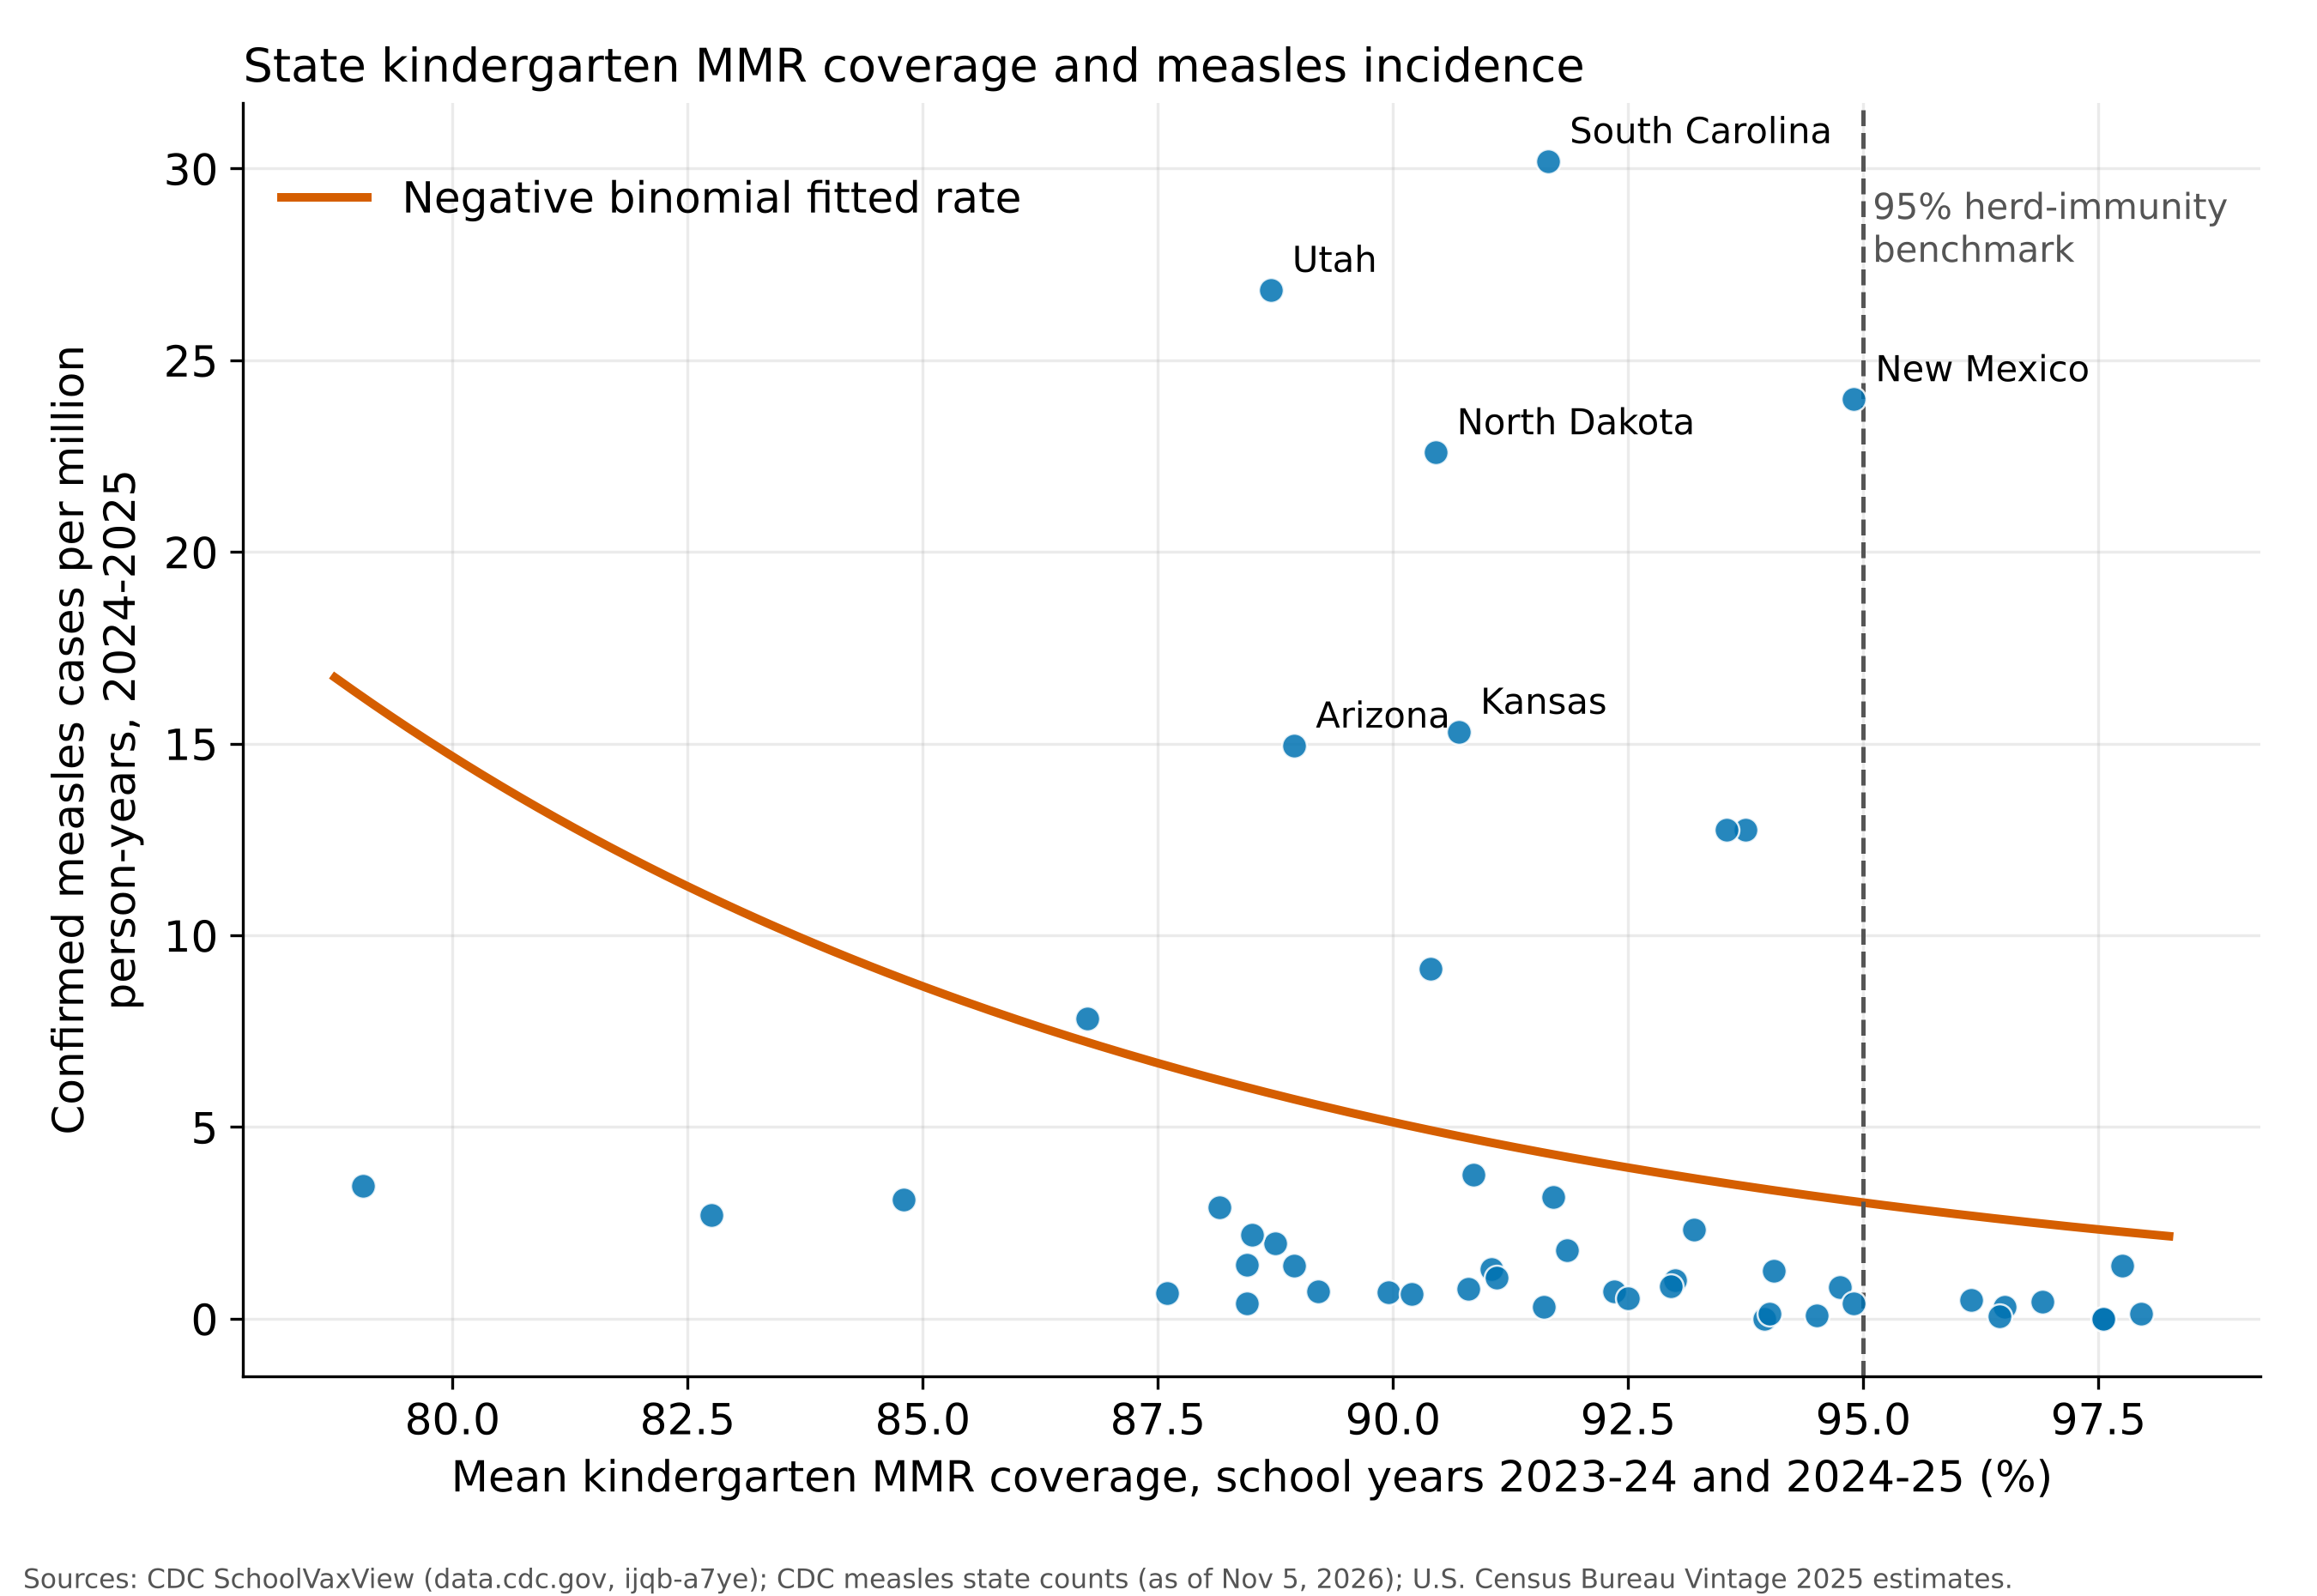
\includegraphics[width=\linewidth]{figures/figure1_mmr_vs_measles.png}
\caption{State kindergarten MMR coverage and measles incidence in the United States. Each point is one jurisdiction (n = 49; Montana and West Virginia lack coverage data). The horizontal axis is mean kindergarten MMR coverage across school years 2023-24 and 2024-25 (percent). The vertical axis is confirmed measles cases per million person-years in 2024 and 2025 combined. The orange curve is the fitted negative binomial model; because a few outbreak states pull the average up, the curve lies above most points. The six jurisdictions with the highest rates and available coverage data are labeled. This is an ecological comparison and does not show causation. Sources: CDC SchoolVaxView; CDC measles state counts as of November 5, 2026; U.S. Census Bureau Vintage 2025 estimates.}
\end{figure}

\begin{table}[H]
\centering\footnotesize
\caption{Associations between kindergarten MMR coverage or non-medical exemption rate and measles cases per million person-years. Spearman $\rho$ with $p$-value; rate ratio (RR) per 1 percentage-point increase with 95\% confidence interval from negative binomial (NB, primary) and Poisson with robust standard errors models. Source: author analysis of CDC and U.S. Census Bureau data.}
\resizebox{\linewidth}{!}{%
\begin{tabular}{lccccc}
\toprule
Comparison & $n$ & Spearman $\rho$ & $p$ & NB RR (95\% CI) & Poisson RR (95\% CI) \\
\midrule
MMR coverage, all & 49 & -0.49 & $<$0.001 & 0.90 (0.78 to 1.04) & 0.94 (0.84 to 1.06) \\
MMR coverage, excluding Texas & 48 & -0.51 & $<$0.001 & 0.88 (0.76 to 1.03) & 0.89 (0.82 to 0.97) \\
Non-medical exemptions, all & 46 & 0.55 & $<$0.001 & 1.20 (1.01 to 1.42) & 1.17 (1.01 to 1.35) \\
Non-medical exemptions, excluding Texas & 45 & 0.57 & $<$0.001 & 1.20 (1.02 to 1.43) & 1.23 (1.06 to 1.42) \\
\midrule
MMR 2023-24 vs.\ 2024 cases & 50 & -0.05 & 0.71 & \multicolumn{2}{c}{not fitted} \\
MMR 2024-25 vs.\ 2025 cases & 49 & -0.49 & $<$0.001 & \multicolumn{2}{c}{not fitted} \\
MMR 2025-26 vs.\ 2026 cases (partial) & 49 & -0.29 & 0.045 & \multicolumn{2}{c}{not fitted} \\
\bottomrule
\end{tabular}%
}
\end{table}

\section*{Discussion}
\subsection*{Principal findings}

Across U.S. jurisdictions, lower kindergarten MMR coverage and higher non-medical exemption rates were moderately associated with more measles cases per million person-years in 2024 and 2025. The rank correlations were consistent in direction and size across several sensitivity analyses. However, the regression estimate for coverage was imprecise and its interval included no association, and the exemption estimate was only modestly above 1. Taken together, the results are suggestive, not conclusive.

The pattern is better described as a tendency than a tight relationship. Some jurisdictions with middling coverage had very high case rates, such as South Carolina (91.7\% coverage), while the three jurisdictions with the lowest coverage (Idaho, Alaska, Wisconsin) had only 2.7 to 3.5 cases per million. This fits how measles outbreaks behave: whether a state has a large outbreak is likely to depend on whether the virus reaches a community with low immunity, which a state average does not capture. Most cases occurred in 2025 and were concentrated in a few jurisdictions: the five with 100 or more cases accounted for 65\% of all cases. With only 269 cases in 2024, the near-zero correlation for that year is unsurprising. The weaker 2026 correlation should be read cautiously because 2026 counts are partial and preliminary.

\subsection*{Comparison with prior work}

The direction of our findings agrees with earlier work linking non-medical exemptions and vaccine refusal to measles and pertussis (Omer et al., 2006, 2009; Phadke et al., 2016) and with models showing that modest drops in coverage could substantially increase cases (Lo \& Hotez, 2017). Those studies used individual-level records, local clustering, or simulation. Our state-level design cannot test those mechanisms, and its weaker model-based evidence is consistent with simulation work showing that state-level averages understate risk when non-vaccination is clustered (Gromis \& Liu, 2022; Masters et al., 2020).

\subsection*{Limitations}

The main limitation is that this is an ecological study. Associations between group averages do not necessarily hold for the individuals or communities within the groups, and ecological estimates can be biased in ways that individual-level studies are not (Greenland \& Robins, 1994; Morgenstern, 1995). We cannot say that unvaccinated children caused or experienced these cases, and CDC data show that many cases were not in kindergarten-age children: in 2025, 26\% of cases were under 5 years, 44\% were 5 to 19, and 29\% were 20 or older (CDC, 2026a). Kindergarten coverage therefore describes only part of each state's immunity.

Second, confounding is likely. Population density, international travel and importation, the presence of close-knit communities, health care access, and differences in testing and reporting may all be associated with both vaccination and measles counts, and we did not adjust for them. Third, the data have measurement limits: coverage is a sample estimate in some states and a census in others, state definitions differ, exemption data are missing for five jurisdictions and coverage for two (including Montana, which had the fifth-highest case rate), and 2025 case counts are preliminary. CDC's state table summed to 269 cases for 2024 against a national 2024 total of 285 on the same page, so some cases were not attributed to a state. Fourth, small counts, with three jurisdictions reporting no cases, make rates unstable. Fifth, the study covers only two years, and results differed by year and by the model used. Finally, the models used custom code that we did not cross-check against another software package, and we did not correct for multiple comparisons.

These limitations suggest what future work should do: use county- or school-level coverage, include several years and covariates, analyze outbreaks as units, and use individual-level case data where available.

\section*{Conclusion}
In 2024 and 2025, lower state kindergarten MMR coverage and higher non-medical exemption rates were moderately associated with higher measles case rates, but the association was imprecise in count models and absent in 2024. State averages are a coarse tool for identifying where measles will spread. Finer-scale vaccination data, and analyses that account for travel, density, and reporting, are needed before these indicators are used to target prevention.

\section*{Data and Code Availability}
All source files, the cleaned dataset, the analysis script, and a results file containing every reported number are openly available at \url{https://github.com/willhhx/measles-vaccination-exemptions-analysis}.

\section*{References}
\begingroup\small\setlength{\parindent}{-0.5in}\setlength{\leftskip}{0.5in}\setlength{\parskip}{4pt}
Centers for Disease Control and Prevention. (2026a). \emph{Measles cases and outbreaks} [Data set]. \url{https://www.cdc.gov/measles/data-research/}

Centers for Disease Control and Prevention. (2026b). \emph{Vaccination coverage and exemptions among kindergartners} [Data set]. \url{https://data.cdc.gov/Vaccinations/Vaccination-Coverage-and-Exemptions-among-Kinderga/ijqb-a7ye}

Greenland, S., \& Robins, J. (1994). Invited commentary: Ecologic studies---biases, misconceptions, and counterexamples. \emph{American Journal of Epidemiology, 139}(8), 747--760. \url{https://doi.org/10.1093/oxfordjournals.aje.a117069}

Gromis, A., \& Liu, K.-Y. (2022). Spatial clustering of vaccine exemptions on the risk of a measles outbreak. \emph{Pediatrics, 149}(1), Article e2021050971. \url{https://doi.org/10.1542/peds.2021-050971}

Guerra, F. M., Bolotin, S., Lim, G., Heffernan, J., Deeks, S. L., Li, Y., \& Crowcroft, N. S. (2017). The basic reproduction number (R0) of measles: A systematic review. \emph{The Lancet Infectious Diseases, 17}(12), e420--e428. \url{https://doi.org/10.1016/S1473-3099(17)30307-9}

Hulland, E. N., Charpignon, M.-L., Berkane, T., \& Majumder, M. S. (2025). Underimmunisation during the 2025 Texas measles outbreak. \emph{The Lancet Infectious Diseases, 25}(6), 607--609. \url{https://doi.org/10.1016/S1473-3099(25)00254-3}

Lo, N. C., \& Hotez, P. J. (2017). Public health and economic consequences of vaccine hesitancy for measles in the United States. \emph{JAMA Pediatrics, 171}(9), 887--892. \url{https://doi.org/10.1001/jamapediatrics.2017.1695}

Masters, N. B., Eisenberg, M. C., Delamater, P. L., Kay, M., Boulton, M. L., \& Zelner, J. (2020). Fine-scale spatial clustering of measles nonvaccination that increases outbreak potential is obscured by aggregated reporting data. \emph{Proceedings of the National Academy of Sciences, 117}(45), 28506--28514. \url{https://doi.org/10.1073/pnas.2011529117}

Morgenstern, H. (1995). Ecologic studies in epidemiology: Concepts, principles, and methods. \emph{Annual Review of Public Health, 16}, 61--81. \url{https://doi.org/10.1146/annurev.pu.16.050195.000425}

Omer, S. B., Enger, K. S., Moulton, L. H., Halsey, N. A., Stokley, S., \& Salmon, D. A. (2008). Geographic clustering of nonmedical exemptions to school immunization requirements and associations with geographic clustering of pertussis. \emph{American Journal of Epidemiology, 168}(12), 1389--1396. \url{https://doi.org/10.1093/aje/kwn263}

Omer, S. B., Pan, W. K. Y., Halsey, N. A., Stokley, S., Moulton, L. H., Navar, A. M., Pierce, M., \& Salmon, D. A. (2006). Nonmedical exemptions to school immunization requirements: Secular trends and association of state policies with pertussis incidence. \emph{JAMA, 296}(14), 1757--1763. \url{https://doi.org/10.1001/jama.296.14.1757}

Omer, S. B., Salmon, D. A., Orenstein, W. A., deHart, M. P., \& Halsey, N. (2009). Vaccine refusal, mandatory immunization, and the risks of vaccine-preventable diseases. \emph{The New England Journal of Medicine, 360}(19), 1981--1988. \url{https://doi.org/10.1056/NEJMsa0806477}

Phadke, V. K., Bednarczyk, R. A., Salmon, D. A., \& Omer, S. B. (2016). Association between vaccine refusal and vaccine-preventable diseases in the United States: A review of measles and pertussis. \emph{JAMA, 315}(11), 1149--1158. \url{https://doi.org/10.1001/jama.2016.1353}

U.S. Census Bureau. (2026). \emph{State population totals and components of change: 2020--2025} (Vintage 2025; file NST-EST2025-ALLDATA.csv) [Data set]. \url{https://www.census.gov/data/tables/time-series/demo/popest/2020s-state-total.html}
\endgroup
\end{document}
